\chapter{Number Representations}

\section{Dot notation}
\paragraph{} 
Extended Dot Notation
\begin{itemize}
	\item Posibit\quad  \(\newmoon\quad\in\quad \{\,\,0,\,\,\,1\}\) 
	\item Negabit\quad	\(\ocircle\quad\in\quad \{-1,0\}\)
	\item Twins
	\begin{enumerate}
		\item Unibit \quad \(\boxdot \quad\in\quad\{\,-1\,,\,1\}\)
		\item Doublebit \quad \(\blacksquare \quad\in\quad\{\,0,\,2\}\)
			\item NegaDoublebit\quad\(\square\quad \in\quad\{\,-2,0\}\)  
	\end{enumerate}

\end{itemize}

Some BSD representation using Extended Dot Notation
\begin{itemize}
	\item \textit{(n,p)} encoding \begin{align*}
		\ocircle\ocircle\ocircle\ocircle\ocircle\\
		\newmoon\,\,\newmoon\,\,\newmoon\,\newmoon\,\newmoon
	\end{align*}
	\item \textit{2's-compl, encoding}
	\begin{align*}
		\square\,\square\,\square\,\square\,\square\\
		\newmoon\,\newmoon\,\newmoon\,\newmoon\,\newmoon
	\end{align*}
	\item  \textit{2's-compl, encoding}
	\begin{align*}
		\ocircle\ocircle\ocircle\ocircle\ocircle\quad\\
		\newmoon\,\,\newmoon\,\,\newmoon\,\newmoon\,\newmoon
	\end{align*}
\end{itemize}
\paragraph{}
Unsigned positive-radix number: \begin{align*}
		\newmoon\,\newmoon\,\newmoon\,\newmoon\,\newmoon\,\newmoon\,\newmoon\,\newmoon
\end{align*}
\textit{2's Complement number}:\begin{align*}
		\ocircle\,\newmoon\,\newmoon\,\newmoon\,\newmoon\,\newmoon\,\newmoon\,\newmoon
\end{align*}
Negative-Radix number:\begin{align*}
		\ocircle\,\newmoon\,\ocircle\,\newmoon\,\ocircle\,\newmoon\,\ocircle\newmoon\,\quad
\end{align*}
Multiplication for signed numbers:
\begin{align*}
	\ocircle\quad\newmoon\quad\newmoon\quad\newmoon \\
	\mathcal{\times}\,\,\ocircle\,\,\,\,\newmoon\quad\newmoon\quad\newmoon\\
	\hline\\
	\ocircle\quad\newmoon\quad\newmoon\quad\newmoon\\
	\ocircle\quad\newmoon\quad\newmoon\quad\newmoon\quad\,\,\,\,\\
	\ocircle\quad\newmoon\quad\newmoon\quad\newmoon\qquad\quad\,\,\\
	\newmoon\quad\ocircle\quad\ocircle\quad\ocircle\quad\qquad\qquad\\
	\hline\\
	\ocircle\quad\newmoon\quad\newmoon\quad\newmoon\quad\newmoon\quad\newmoon\quad\newmoon\quad\newmoon
\end{align*}\\

Addition for unsigned positive-radix numbers:
\begin{align*}
	\ocircle\quad\newmoon\quad\newmoon\quad\newmoon \,\\
	\textbf{+}\quad\ocircle\quad\newmoon\quad\newmoon\quad\newmoon\\
	\hline
	\quad\ocircle\quad\newmoon\quad\newmoon\quad\newmoon\,\,\,\,\,\newmoon
\end{align*}\\
Multiplication for unsigned positive-radix numbers:
\begin{align*}
	\newmoon\quad\newmoon\quad\newmoon \\
	\mathcal{\times}\quad\newmoon\quad\newmoon\quad\newmoon\\
	\hline\\
	\newmoon\quad\newmoon\quad\newmoon\quad\newmoon\\
	\newmoon\quad\newmoon\quad\newmoon\quad\newmoon\quad\quad\\
	\newmoon\quad\newmoon\quad\newmoon\quad\newmoon\qquad\qquad\\
	\newmoon\quad\newmoon\quad\newmoon\quad\newmoon\qquad\qquad\qquad\\
	\hline\\
	\newmoon\quad\newmoon\quad\newmoon\quad\newmoon\quad\newmoon\quad\newmoon\quad\newmoon\quad\newmoon
\end{align*}\\
Addition for unsigned positive-radix numbers:
\begin{align*}
	\newmoon\quad\newmoon\quad\newmoon \\
	\textbf{+}\quad\newmoon\quad\newmoon\quad\newmoon\\
	\hline\\
	\quad\newmoon\quad\newmoon\quad\newmoon\quad\newmoon
\end{align*}\\
\\
There are many other number representations but the most important ones are:
\begin{enumerate}
	\item \textbf{2's} Complement
	\item \textbf{Binary Stored-carry} or \textbf{Carry-saved} format
	\item \textbf{Binary floating point number } (IEEE 754)
	\item \textbf{BCD}
\end{enumerate}

\section{Signed Number Representations}
\subsection{Signed-Magnitude Representation}
Definition: The \textbf{most left bit} is the \textbf{sign bit} (s) \[
	\mathbf{if}
\left\{\begin{array}{cl}
	s\,=\,0 & \Longrightarrow \text{positive number}\\s\,=1 & \Longrightarrow \text{negative number} 
\end{array}\right\}
\]
Numbers of this Representation type are \textit{fix-point and with no fraction}\\
In \textit{Radix r} the number \(k\)  of digits needed for representing [0,max] is
\[
	k\,=\,\left\lfloor\,log_{r}max\,+\,1 \right\rfloor\,+1\,=\,\left\lceil log_{r}(max+1) \right\rceil 
\]
\\
Example: for Radix=2 and range is [0,7] how many digits are needed?
\\\\Solution: \(k\,=\left\lceil log_{2}(7+1) \right\rceil \Longrightarrow\, 3\) so there are 3 digits are needed for representing this digit set\\\\
\textbf{Disadvantages of Signed-Magnitude Representation}
\begin{enumerate}
	\item Because of Symmetric nature of this representation there will be two \(0\)s with different signs \(\pm0\). This is unavoidable in Radix-2 Symmetric Systems.
	\item More overhead and thus more delay because of \(\pm0\) existence.
\end{enumerate}
Finally the Digit set of \textbf{Signed-Magnitude Representation} is 
\[
	\big[-(2^{k-1}\,-\,1)\,,2^{k\,-\,1}\,-1\big]
\]
\begin{figure*}
	\centering
	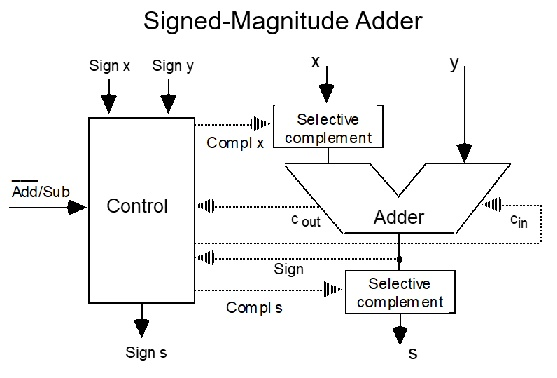
\includegraphics{smadder.jpg}
	\caption[short]{Adding signed-magnitude numbers using precomplementation and postcomplementation.}
\end{figure*}

\subsection{Biased Representations}
\paragraph{}
As the name suggests\textit{\textbf{ a bias}} is applied to the \textbf{signed number}; which then can be used for conversion from\textbf{ Signed} to \textbf{Unsigned} numbers.\\
The\textbf{ Digit set }can be shown as \( \mathbf{{[-bias,max-bias}]} \); using values from \textbf{0} to \textbf{max}, this is often called \textbf{"excess-bias"}. Most notable examples are \textbf{"excess-3" or (BCD)} and \textbf{"excess-128"} (is used for simpler hardware) coding.
Formula Demonstration:\begin{align*}
	x+y-bias=(x+bias)+(y+bias)-bias \\
	x-y+bias=(x+bias)-(y+bias)+bias\\
	\text{with kbit numbers and  a bias of } \mathbf{2^{k-1}}
\end{align*}
The Complexity is\textbf{ negligible} for this type.\\
Multiplications and Divisions become \textit{more difficult} if applied on \textbf{biased numbers}, thus the \textit{bias representation} is mostly suited for the \textbf{exponent (e)} part of \textbf{the floating-point numbers}, since they are \underline{\textbf{never}} multiplied or divided. A common example of this is \textbf{IEEE 754 standard}.